
\begin{tikzpicture}
  \begin{axis}[
    ybar stacked,
    % ybar interval=0.7,
    % grid=x,
    width=9cm, height=6cm,
    xtick=data,
    ytick distance=2,
    ymajorgrids=true,
    yminorgrids=true,
    minor y tick num=1,
    ymin=0,
    ymax=10,
    axis on top,
    grid style={draw=white,line width=0.5mm},
    ]
\only<1->{\addplot[draw=green,fill=green] coordinates {(0,1)(1,1)(2,1)(3,1)(4,1)};}
\only<2>{\addplot[draw=blue,fill=blue] coordinates {(0, 0)(1, 0)(2, 0)(3, 0)(4, 1)};}
\only<3>{\addplot[draw=blue,fill=blue] coordinates {(0, 0)(1, 0)(2, 0)(3, 1)(4, 1)};}
\only<4>{\addplot[draw=blue,fill=blue] coordinates {(0, 0)(1, 0)(2, 0)(3, 2)(4, 1)};}
\only<5>{\addplot[draw=blue,fill=blue] coordinates {(0, 0)(1, 0)(2, 0)(3, 3)(4, 1)};}
\only<6>{\addplot[draw=blue,fill=blue] coordinates {(0, 1)(1, 0)(2, 0)(3, 3)(4, 1)};}
\only<7>{\addplot[draw=blue,fill=blue] coordinates {(0, 1)(1, 0)(2, 0)(3, 4)(4, 1)};}
\only<8>{\addplot[draw=blue,fill=blue] coordinates {(0, 1)(1, 0)(2, 0)(3, 5)(4, 1)};}
\only<9>{\addplot[draw=blue,fill=blue] coordinates {(0, 1)(1, 0)(2, 0)(3, 6)(4, 1)};}
\only<10>{\addplot[draw=blue,fill=blue] coordinates {(0, 1)(1, 0)(2, 0)(3, 7)(4, 1)};}
\only<11>{\addplot[draw=blue,fill=blue] coordinates {(0, 1)(1, 0)(2, 1)(3, 7)(4, 1)};}
\only<12>{\addplot[draw=blue,fill=blue] coordinates {(0, 1)(1, 0)(2, 1)(3, 7)(4, 2)};}

  \end{axis}
\end{tikzpicture}
